\capitolo{Dimensionamento e Scelta di Viti a Ricircolo di Sfere}
I riduttori vite madrevite classici sono a strisciamento e questa caratteristica li rende particolarmente soggetti all'attrito, quindi a ridotto rendimento e irreversibilità del moto. Queste sono caratteristiche desiderabili per strutture, meno per organi in moto, si fa largo la necessità di rendimenti superiori, quindi vengono utilizzate tecnologie differenti.

La principale delle tecnologie alternative è quella di riduttori a vite a ricircolo di sfere in cui lo spostamento viene trasmesso dalle sfere che rotolando permettono di avere ridotto attrito, quindi rendimento maggiore, indicativamente \( \eta_{R\rightarrow T} \simeq 0.97 \simeq \eta_{T\rightarrow R} \).

Le sfere sono poste all'interno di gole su cui possono scorrere, presenti al posto dei denti nella vite e madrevite, chiamata in questo contesto chiocciola.

\paragrafo{Configurazioni cinematiche:}
In termmini di cinematica le viti a ricircolo di sfere sono equivalenti alle viti-madreviti a strisciamento, in particolare vale ancora \( \tau_v = \frac{p}{2\pi} = \frac{\Delta x_{rel}}{\Delta \theta_{rel}} \), dove gli spostamenti sono considerati relativi.
In seguito sono rappresentate le varie combinazioni di movimenti assoluti.

\begin{figure}[h]
    \centering
    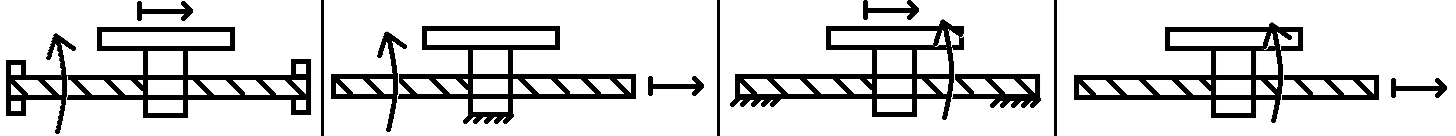
\includegraphics[width=0.9\textwidth]{Immagini/confi_din_vite_ricircolo.png}
    \caption{4 possibili configurazioni rotazione-traslazione relative}
\end{figure}

\sezione{Parametri di scelta}
La scelta di viti a ricircolo di sfere non è banale perché ha dipendenza da un alto numero di combinazioni possibili di diametri viti e sfere, passo della vite, vita utile, numero di principi e tipologia di materiali.

\paragrafo{Numero di principi:}
Con numero di principi si intendono i singoli percorsi indipendenti di ricircolo delle sfere. All'interno di un passo della vite potrebbe esserci sufficiente spazio per inserire un ulteriore ricircolo di sfere, così nasce una vite a due principi.

\sottosezione{Dinamica}
Similmente a come visto per i riduttori si vanno a definire la forza applicata sul carico: \( C_m = \left( J_m + J_v + M \frac{\tau_v^2}{\eta_v} \right) \AccAng_m + F \frac{\tau_v}{\eta_v} \), da cui, a seguito di opportuna manipolazione, si ottiene: \( C_m = \left(J_m + J_v\right) \frac{\Ddot x}{\tau_v} + \frac{\tau_v}{\eta_v} \left( M\Ddot x + F \right) \), dove:
\[ F_a = M\Ddot x + F \]
risultante delle forze assiali applicate alla chiocciola (equivalente a \( T_2 \) dei riduttori).

\begin{figure}[h]
    \centering
    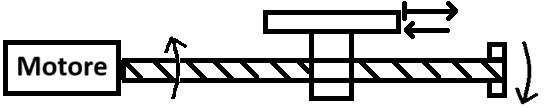
\includegraphics[width=0.4\textwidth]{Immagini/mot_vite_ricircolo.png}
    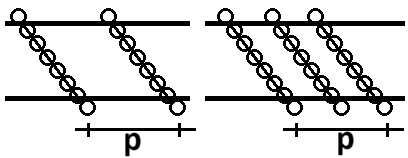
\includegraphics[width=0.3\textwidth]{Immagini/principi_viti_ricircolo.png}
    \caption{Schema motore e vite a ricircolo di sfere sx; Uno vs Due principi dx}
\end{figure}

\sottosottosezione{Forza assiale media}
Anche in questo caso nel regime stazionario si fanno valutazioni sulla media, e in modo simile a \( T_{2,media} \) si ottiene:
\[ F_{a, media} = \sqrt[3]{\frac{\int^{T_{ciclo}}_0 \abs{F_a^3(t)\Ddot{x}_c(t)dt}}{\int^{T_{ciclo}}_0 \abs{\Ddot{x}_c(t)}dt}} \]
E anche in questo caso per moto ad andamento trapezoidale l'integrale diventerà una sommatoria.

\sottosottosezione{Capacità di Carico Dinamico}
Per capacità di carico dinamico \( C_D [N] \) si intende nei cataloghi la forza assiale applicata alla  chiocciola che garantisce con probabilità di sopravvivenza del \(90\%\) la vita utile di \(10^6\) giri relativi vite-chiocciola.

\paragrafo{Migliorare la probabilità:}
Per migliorare la probabilità occorre utilizzare un fattore di affidabilità \(<1\) che vada a penalizzare il valore a catalogo. Si tratta di valori ricavati statisticamente, non hanno significato di coefficiente di sicurezza.

\paragrafo{Utilizzo di CCD in verifica:}
Noti \(C_D, F_{a, media}\), volendo calcolare la vita utile della chiocciola per il \(90\%\) di probabilità di sopravvivenza si utilizza la formula di Wohler: \( C_D^3 10^6 = F_{a,media}^3 L_N \), con \(L_N\) vita utile in termini di numero di rotazioni.

\paragrafo{Utilizzo di CCD in dimensionamento:}
Noto \(F_{a,media}\), data dalla specifica in termini di giri sulla vita utile \(L_N^{des}\) desiderata, è possibile calcolare \(C_D\) idoneo a garantire la vita desiderata al \(x\%\) invertendo la formula e utilizzando un opportuno fattore di affidabilità.

\paragrafo{Vita utile in ore:}
Solitamente non è nota la vita utile in numero di giri relativi, è più comodo passare in ore di lavoro, quindi 
\[ L_H = L_N \frac{1}{\VelAng_v} \frac{1}{60} [h] = L_N \frac{p}{3600 \cdot \dot{x}_{media}} \]
che si traduce in una CCD richiesta: 
\[ C_{D,rich} \geqslant F_{a,media} \sqrt[3]{\frac{L_H^{des}\dot{x}^{des} \cdot 3600}{p \cdot 10^6}} f_s \]

\sottoparagrafo{Fattore di Shock/Servizio:}
Alla CCD in esame va moltiplicato un fattore di shock o servizio \( f_s \), i cui valori possono cambiare tra \( 1.2 \div 3 \), se possibile conviene utilizzare un modello elasto-dinamico per avere una idea delle forze in gioco e evitare di sovradimensionare la chiocciola.

\paragrafo{Dipendenze della CCD richiesta:}
La CCD è dipendente direttamente da velocità traslante e vita utile, mentre è inversamente dipendente dal passo \( p \downarrow, C_D \uparrow\). La dipendenza inversa del passo risulta chiara immaginando che i passi minori portano a un maggior numero di giri relativi a pari velocità.

\paragrafo{Dipendenze della CCD:}
Il carico dinamico sulla chiocciola dipende principalmente dal volume delle sfere e dal materiale delle stesse, quindi maggiore lo spazio disponibile alle sfere meglio è, perciò aumenta con il diametro delle viti \(d_v\), con l'utilizzo di sfere di raggio maggiore e l'utilizzo di viti a più principi.
Come regola generale conviene avere meno sfere più grandi che tenderanno a raggiungere un volume complessivo maggiore, inoltre garantiscono una maggior resistenza.

\begin{figure}[h]
    \centering
    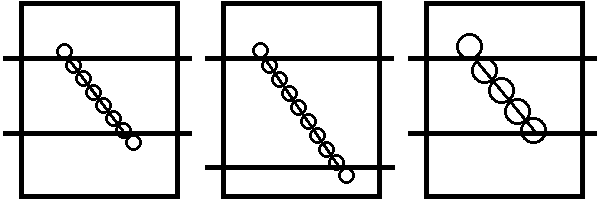
\includegraphics[width=0.4\textwidth]{Immagini/CCD_chiocciola_sfere.png}
    \caption{Dipendenza volume sfere}
\end{figure}

\sottosezione{Velocità limite delle sfere}
Durante il moto le sfere ruotano tra le due gole di vite e chiocciola, ma in questo movimento vanno anche a strisciare tra loro. Per velocità elevate risulta un aumento di riscaldamento e un aumento usura legato alla formazione di particolato di sfere.
La relazione da verificare è \( v_{sfere} = \VelAng_v \frac{d}{2} < v_{lim} \) dove \(d\) è la distanza tra centri delle due sfere opposte, e con velocità limite specifica della chiocciola.

Nei cataloghi non si tiene conto della velocità della sfera, ma del doppio, e viene chiamata "D \(\times\) n" \(= \VelAng_v\cdot d \), quindi  il limite diventa: \(d \cdot \VelAng_v < \text{"D}\times \text{n"}_{lim} \alpha = S \).

\sottosottosezione{Sfere di Acciaio e Ceramica}
In alternativa alle sfere solo di acciaio, esistono viti a ricircolo di sfere in cui sono alternate sfere di acciaio e di ceramica. In particolare le seconde oltre a essere costruite con un volume leggermente inferiore, hanno una massa inferiore, perciò quando vengono messe in movimento le sfere di acciaio quelle di ceramica vanno in contro-rotazione, così facendo il contatto tra sfere vede anch'esso rotazione, mentre permane lo strisciamento sui punti di contatto tra sfere cercamiche e gola. Questa configurazione permette di raggiungere velocità limite della singola sfera \( \DperN_{lim} \) molto superiori, anche doppi.

\begin{figure}[h]
    \centering
    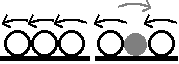
\includegraphics[width=0.2\textwidth]{Immagini/Viti_A_C.png}
    \caption{Viti a ricircolo di sfere in acciaio e ceramica}
\end{figure}

\sottosottosezione{Vincolo 1 su p,d}
A partire da \( d\cdot \VelAng_v \leqslant S = \DperN_{lim} \alpha \), sostituendo la velocità della vite con la velocità del carico traslante, ed esplicitando il passo della vite, si ottiene una relazione di vincolo per passo e diametro della vite:
\[ p \geqslant \frac{\Ddot{x_{max}} 2\pi }{S} d \]

Nota bene che \(\Ddot{x_{max}}\) solitamente non è un dato progettuale, è possibile sceglierlo entro limiti termici/strutturali.

\sottosezione{Velocità critica della vite}
La vite è naturalmente sbilanciata, ruotando crea una forzante armonica alla frequenza della velocità di rotazione \( \VelAng_v \), che di valori prossimi alla velocità naturale flessionale \(\omega_{N,flex}\) porta ad avere forti vibrazioni.
Per ridurre gli effetti delle vibrazioni si possono adottare due soluzioni.

\sottosottosezione{Viti smorzate}
Per limitare le vibrazioni è possibile utilizzare viti con un anima in elastomero che vada a smorzare le vibrazioni, inoltre essendo al centro del diametro della vite non andrà a comprometterne la rigidità. Valori tipici di smorzamento di viti smorzate sono \(\epsilon \simeq 0.3 \div 0.5\), contro i \(\epsilon \simeq 0.0x \) di viti normali.

\sottosottosezione{Limitare la velocità di rotazione}
Per evitare di ottenere sulla vite vibrazioni elevate basta evitare di passare per frequenze naturali, cioè \( \VelAng_v < \omega_{N,flex}(x) \), dove \( \omega_{N,flex}(x) \) è dipendente dalla posizione in cui si trova la chiocciola, perché questa solitamente scorre su di una guida in modo da evitare sia la vite a dover sopportare il peso del carico, e quindi va ad aumentare la rigidezza localmente. Il problema risulta complicato.

\paragrafo{Applicazioni velocità in funzione di x:}
Noto il modello elastodinamico della vite, o effettuate opportune misurazioni, è possibile ottenere l'andamento della pulsazione naturale per le varie posizioni della chiocciola \(x\), quindi è possibile variare la  velocità massima della vite in funzione di \(x\). Non semplice.

\paragrafo{Approccio conservativo:}
In alternativa è possibile utilizzare un approccio conservativo in cui si va a limitare la velocità della vite alla minore delle pulsazioni naturali flessionali \( \VelAng_v < \omega_{N,flex}^{min} \). Non è la soluzione ottimale.

Considerando la massa della sola vite\footnote{Carico e madrevite andranno a gravare sulla guida.} la pulsazione naturale flessionale vale:
\[ \omega_{N,flex} = K_v \sqrt{\frac{E \cdot I_f}{M_v \cdot L^3}} \]
con \( K_v \) coefficiente legato al tipo di vincolo; \( E \) modulo di Joung del materiale; \( I_f = \frac{\pi}{64}d^4 \) momento di inerzia; \( M_v \) massa della vite; \( L \) lunghezza della vite.

\sottoparagrafo{Coefficiente di vincolo:}
Il coefficiente di vincolo dipende dal tipo di vincolo presente all'estremo della vite, può essere: libero; appoggio; incastro\footnote{Nota bene non è un incastro di tipo strutturale, è un incastro solo in termini flessionali, non necessariamente andrà a limitare la rotazione della vite.}.
Queste tre possibilità risultano in 4 combinazioni:
\begin{itemize}
    \item Incastro + Libero: \(K_v = 3.5\)
    \item Appoggio + Appoggio: \(K_v = \pi^2\)
    \item Appoggio + Incastro: \(K_v = 15.4\), soluzione preferita.
    \item Incastro + Incastro: \(K_v = 22.4\), questa è la soluzione col coeffiente maggiore. Tuttavia se la vite si riscalda e quindi si dilata, tende a spanciare; inoltre richiede montaggio preciso.
\end{itemize}

\sottoparagrafo{Vincolo 2 su p,d:}
A partire dalla disequazione \( \VelAng_v^{max} \geqslant \omega_{N,flex}^{min} \alpha \), con \( \alpha \simeq 0.6\div 0.8 \) coefficiente di sicurezza che considera come l'ampiezza inizi a salire prima del valore esatto di pulsazione naturale, sostituisco i vari elementi, effettuo qualche manipolazione e si ottiene:
\[ p \leqslant \frac{8\pi L^2 \Ddot{x}^{max} \sqrt{\rho}}{K_v \alpha \sqrt{E}} \cdot \frac{1}{d} \]
Disequazione per cui risulta evidente la dipendenza inversa tra passo e diametro; quindi che per velocità superiori il vincolo peggiora; che per lunghezze superiori il vincolo peggiora quadraticamente; che per coefficienti di vincoli inferiori il vincolo peggiora.

\begin{figure}[h]
    \centering
    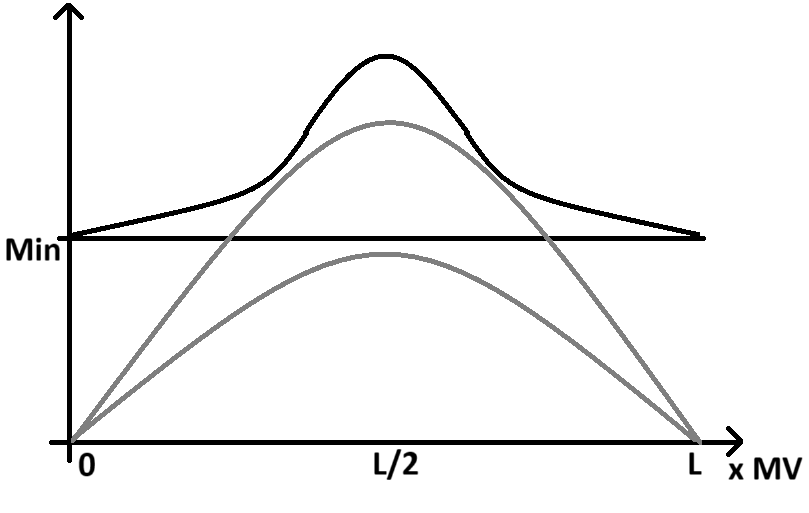
\includegraphics[width=0.4\textwidth]{Immagini/vel_critica_vite_2sol.png}
    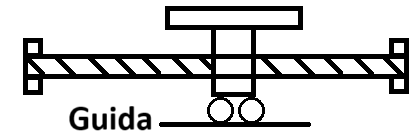
\includegraphics[width=0.3\textwidth]{Immagini/vite_guida_MV.png}
\end{figure}

\sottosezione{Vincoli su passo e diametro della vite}
Andando a unire i due vincoli ricavati: \(p \geqslant \frac{\Ddot{x_{max}} 2\pi }{S} d\) e \( p \leqslant \frac{8\pi L^2 \Ddot{x}^{max} \sqrt{\rho}}{K_v \alpha \sqrt{E}} \cdot \frac{1}{d} \), la curva ottenuta sarà come in figura. Va evidenziato il forte limite per diametri ridotti.

\sottosottosezione{Esempio}
Fosse richiesto un \( C_D \) "basso", e quindi occorra utilizzare \(d\) "piccoli". In questo caso utilizzare viti acciaio e ceramica non ha senso, perché andrebbe a influenzare unicamente valori di diametro superiori. In questo caso utilizzare vincoli più rigidi potrebbe aiutare, perché porterebbero ad un aumento del numero di punti utilizzabili, tuttavia occorre valutare se i valori aggiunti possano essere utilizzati nell'applicazione in esame o meno.

\begin{figure}[h]
    \centering
    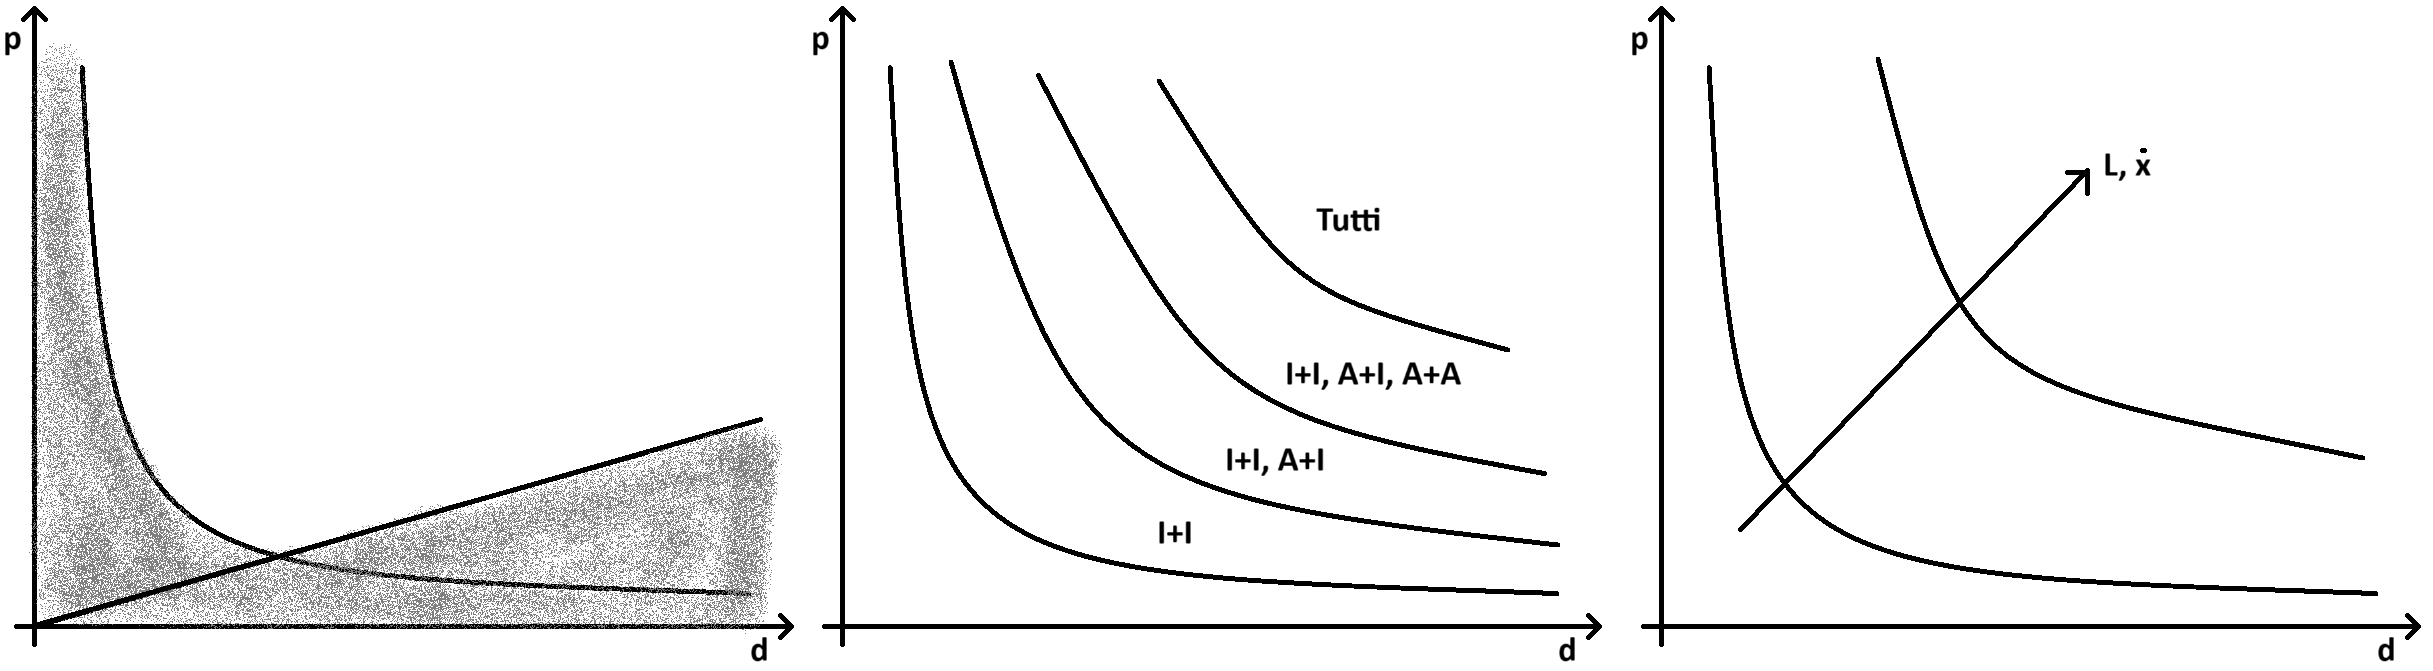
\includegraphics[width=0.75\textwidth]{Immagini/viti_ricir_vincoli_p_d.png}
    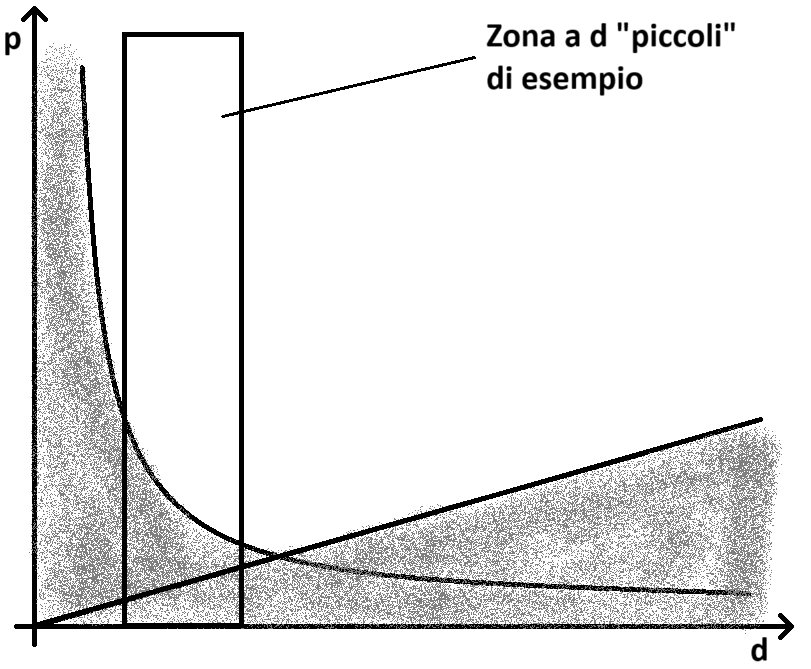
\includegraphics[width=0.25\textwidth]{Immagini/viti_ricir_esempio_vincoli.png}
    \caption{1-3 relative a vincolo e dipendenze, 4 relativa all'esempio}
\end{figure}
% inserire immagini di esempio di unione vincoli e esercizio